
\documentclass[letterpaper,hide notes,xcolor={table,svgnames},pdftex,10pt]{beamer}
\def\showexamples{t}


%\usepackage[svgnames]{xcolor}

%% Demo talk
%\documentclass[letterpaper,notes=show]{beamer}

\usecolortheme{crane}
\setbeamertemplate{navigation symbols}{}

\usetheme{MyPittsburgh}
%\usetheme{Frankfurt}

%\usepackage{tipa}

\usepackage{hyperref}
\usepackage{graphicx,xspace}
\usepackage[normalem]{ulem}
\usepackage{multicol}
\usepackage{amsmath,amssymb,amsthm,graphicx,xspace}
\newcommand\SF[1]{$\bigstar$\footnote{SF: #1}}

\usepackage[default]{sourcesanspro}
\usepackage[T1]{fontenc}
\usepackage[scaled]{beramono}
\usepackage{tikzpagenodes}

\newcounter{tmpnumSlide}
\newcounter{tmpnumNote}


% old question code
%\newcommand\question[1]{{$\bigstar$ \small \onlySlide{2}{#1}}}
% \newcommand\nquestion[1]{\ifdefined \presentationonly \textcircled{?} \fi \note{\par{\Large \textbf{?}} #1}}
% \newcommand\nanswer[1]{\note{\par{\Large \textbf{A}} #1}}


 \newcommand\mnote[1]{%
   \addtocounter{tmpnumSlide}{1}
   \ifdefined\showcues {~\tiny\fbox{\arabic{tmpnumSlide}}}\fi
   \note{\setlength{\parskip}{1ex}\addtocounter{tmpnumNote}{1}\textbf{\Large \arabic{tmpnumNote}:} {#1\par}}}

\newcommand\mmnote[1]{\note{\setlength{\parskip}{1ex}#1\par}}

%\newcommand\mnote[2][]{\ifdefined\handoutwithnotes {~\tiny\fbox{#1}}\fi
% \note{\setlength{\parskip}{1ex}\textbf{\Large #1:} #2\par}}

%\newcommand\mnote[2][]{{\tiny\fbox{#1}} \note{\setlength{\parskip}{1ex}\textbf{\Large #1:} #2\par}}

\newcommand\mquestion[2]{{~\color{red}\fbox{?}}\note{\setlength{\parskip}{1ex}\par{\Large \textbf{?}} #1} \note{\setlength{\parskip}{1ex}\par{\Large \textbf{A}} #2\par}\ifdefined \presentationonly \pause \fi}

\newcommand\blackboard[1]{%
\ifdefined   \showblackboard
  {#1}
  \else {\begin{center} \fbox{\colorbox{blue!30}{%
         \begin{minipage}{.95\linewidth}%
           \hspace{\stretch{1}} Some space intentionally left blank; done at the blackboard.%
         \end{minipage}}}\end{center}}%
         \fi%
}



%\newcommand\q{\tikz \node[thick,color=black,shape=circle]{?};}
%\newcommand\q{\ifdefined \presentationonly \textcircled{?} \fi}

\usepackage{listings}
\lstset{basicstyle=\footnotesize\ttfamily,
	breaklines=true,
	aboveskip=15pt,
  	belowskip=15pt,
	frame=lines,
	numbers=left, basicstyle=\scriptsize, numberstyle=\tiny, stepnumber=0, numbersep=2pt
}

\usepackage{siunitx}
\newcommand\sius[1]{\num[group-separator = {,}]{#1}\si{\micro\second}}
\newcommand\sims[1]{\num[group-separator = {,}]{#1}\si{\milli\second}}
\newcommand\sins[1]{\num[group-separator = {,}]{#1}\si{\nano\second}}
\sisetup{group-separator = {,}, group-digits = true}

%% -------------------- tikz --------------------
\usepackage{tikz}
\usetikzlibrary{positioning}
\usetikzlibrary{arrows,backgrounds,automata,decorations.shapes,decorations.pathmorphing,decorations.markings,decorations.text,decorations.pathreplacing}

\tikzstyle{place}=[circle,draw=blue!50,fill=blue!20,thick, inner sep=0pt,minimum size=6mm]
\tikzstyle{transition}=[rectangle,draw=black!50,fill=black!20,thick, inner sep=0pt,minimum size=4mm]

\tikzstyle{block}=[rectangle,draw=black, thick, inner sep=5pt]
\tikzstyle{bullet}=[circle,draw=black, fill=black, thin, inner sep=2pt]

\tikzstyle{pre}=[<-,shorten <=1pt,>=stealth',semithick]
\tikzstyle{post}=[->,shorten >=1pt,>=stealth',semithick]
\tikzstyle{bi}=[<->,shorten >=1pt,shorten <=1pt, >=stealth',semithick]

\tikzstyle{mut}=[-,>=stealth',semithick]

\tikzstyle{treereset}=[dashed,->, shorten >=1pt,>=stealth',thin]

\usepackage{ifmtarg}
\usepackage{xifthen}
\makeatletter
% new counter to now which frame it is within the sequence
\newcounter{multiframecounter}
% initialize buffer for previously used frame title
\gdef\lastframetitle{\textit{undefined}}
% new environment for a multi-frame
\newenvironment{multiframe}[1][]{%
\ifthenelse{\isempty{#1}}{%
% if no frame title was set via optional parameter,
% only increase sequence counter by 1
\addtocounter{multiframecounter}{1}%
}{%
% new frame title has been provided, thus
% reset sequence counter to 1 and buffer frame title for later use
\setcounter{multiframecounter}{1}%
\gdef\lastframetitle{#1}%
}%
% start conventional frame environment and
% automatically set frame title followed by sequence counter
\begin{frame}%
\frametitle{\lastframetitle~{\normalfont(\arabic{multiframecounter})}}%
}{%
\end{frame}%
}
\makeatother

\makeatletter
\newdimen\tu@tmpa%
\newdimen\ydiffl%
\newdimen\xdiffl%
\newcommand\ydiff[2]{%
    \coordinate (tmpnamea) at (#1);%
    \coordinate (tmpnameb) at (#2);%
    \pgfextracty{\tu@tmpa}{\pgfpointanchor{tmpnamea}{center}}%
    \pgfextracty{\ydiffl}{\pgfpointanchor{tmpnameb}{center}}%
    \advance\ydiffl by -\tu@tmpa%
}
\newcommand\xdiff[2]{%
    \coordinate (tmpnamea) at (#1);%
    \coordinate (tmpnameb) at (#2);%
    \pgfextractx{\tu@tmpa}{\pgfpointanchor{tmpnamea}{center}}%
    \pgfextractx{\xdiffl}{\pgfpointanchor{tmpnameb}{center}}%
    \advance\xdiffl by -\tu@tmpa%
}
\makeatother
\newcommand{\copyrightbox}[3][r]{%
\begin{tikzpicture}%
\node[inner sep=0pt,minimum size=2em](ciimage){#2};
\usefont{OT1}{phv}{n}{n}\fontsize{4}{4}\selectfont
\ydiff{ciimage.south}{ciimage.north}
\xdiff{ciimage.west}{ciimage.east}
\ifthenelse{\equal{#1}{r}}{%
\node[inner sep=0pt,right=1ex of ciimage.south east,anchor=north west,rotate=90]%
{\raggedleft\color{black!50}\parbox{\the\ydiffl}{\raggedright{}#3}};%
}{%
\ifthenelse{\equal{#1}{l}}{%
\node[inner sep=0pt,right=1ex of ciimage.south west,anchor=south west,rotate=90]%
{\raggedleft\color{black!50}\parbox{\the\ydiffl}{\raggedright{}#3}};%
}{%
\node[inner sep=0pt,below=1ex of ciimage.south west,anchor=north west]%
{\raggedleft\color{black!50}\parbox{\the\xdiffl}{\raggedright{}#3}};%
}
}
\end{tikzpicture}
}


%% --------------------

%\usepackage[excludeor]{everyhook}
%\PushPreHook{par}{\setbox0=\lastbox\llap{MUH}}\box0}

%\vspace*{\stretch{1}

%\setbox0=\lastbox \llap{\textbullet\enskip}\box0}

\setlength{\parskip}{\fill}

\newcommand\noskips{\setlength{\parskip}{1ex}}
\newcommand\doskips{\setlength{\parskip}{\fill}}

\newcommand\xx{\par\vspace*{\stretch{1}}\par}
\newcommand\xxs{\par\vspace*{2ex}\par}
\newcommand\tuple[1]{\langle #1 \rangle}
\newcommand\code[1]{{\sf \footnotesize #1}}
\newcommand\ex[1]{\uline{Example:} \ifdefined \presentationonly \pause \fi
  \ifdefined\showexamples#1\xspace\else{\uline{\hspace*{2cm}}}\fi}

\newcommand\ceil[1]{\lceil #1 \rceil}


\AtBeginSection[]
{
   \begin{frame}
       \frametitle{Outline}
       \tableofcontents[currentsection]
   \end{frame}
}



\pgfdeclarelayer{edgelayer}
\pgfdeclarelayer{nodelayer}
\pgfsetlayers{edgelayer,nodelayer,main}

\tikzstyle{none}=[inner sep=0pt]
\tikzstyle{rn}=[circle,fill=Red,draw=Black,line width=0.8 pt]
\tikzstyle{gn}=[circle,fill=Lime,draw=Black,line width=0.8 pt]
\tikzstyle{yn}=[circle,fill=Yellow,draw=Black,line width=0.8 pt]
\tikzstyle{empty}=[circle,fill=White,draw=Black]
\tikzstyle{bw} = [rectangle, draw, fill=blue!20, 
    text width=4em, text centered, rounded corners, minimum height=2em]
    
    \newcommand{\CcNote}[1]{% longname
	This work is licensed under the \textit{Creative Commons #1 3.0 License}.%
}
\newcommand{\CcImageBy}[1]{%
	\includegraphics[scale=#1]{creative_commons/cc_by_30.pdf}%
}
\newcommand{\CcImageSa}[1]{%
	\includegraphics[scale=#1]{creative_commons/cc_sa_30.pdf}%
}
\newcommand{\CcImageNc}[1]{%
	\includegraphics[scale=#1]{creative_commons/cc_nc_30.pdf}%
}
\newcommand{\CcGroupBySa}[2]{% zoom, gap
	\CcImageBy{#1}\hspace*{#2}\CcImageNc{#1}\hspace*{#2}\CcImageSa{#1}%
}
\newcommand{\CcLongnameByNcSa}{Attribution-NonCommercial-ShareAlike}

\newenvironment{changemargin}[1]{% 
  \begin{list}{}{% 
    \setlength{\topsep}{0pt}% 
    \setlength{\leftmargin}{#1}% 
    \setlength{\rightmargin}{1em}
    \setlength{\listparindent}{\parindent}% 
    \setlength{\itemindent}{\parindent}% 
    \setlength{\parsep}{\parskip}% 
  }% 
  \item[]}{\end{list}} 



\usepackage{multirow}

\title{Lecture 13 --- Dependencies and Speculation }

\author{Patrick Lam \& Jeff Zarnett \\ \small \texttt{patrick.lam@uwaterloo.ca}, \texttt{jzarnett@uwaterloo.ca}}
\institute{Department of Electrical and Computer Engineering \\
  University of Waterloo}
\date{\today}


\begin{document}

\begin{frame}
  \titlepage

 \end{frame}

%%%%%%%%%%%%%%%%%%%%%%%%%%%%%%%%%%%%%%%%%%%%%%%%%%%%%%%%%%%%%%%%%%%%%%%%%%%%%%%%
\begin{frame}
  \frametitle{Next topic: Dependencies}

\begin{center}
	
\includegraphics[width=0.4\textwidth]{images/dependency.jpeg}
\end{center}

     \structure{Dependencies} are the main
      limitation to parallelization.\\[1em]
     Example: computation must be evaulated as {\tt XY} and not {\tt YX}.\\[1em]
  
\end{frame}

\begin{frame}
  \frametitle{Not synchronization}

  
      Assume (for now) no synchronization problems.\\[1em]
      Only trying to identify code that is safe to run in
      parallel.

  
\end{frame}
%%%%%%%%%%%%%%%%%%%%%%%%%%%%%%%%%%%%%%%%%%%%%%%%%%%%%%%%%%%%%%%%%%%%%%%%%%%%%%%%

\begin{frame}
\frametitle{Dependencies: Analogies}

Must extract bicycle from garage before closing garage door.

Must close washing machine door before starting the cycle.

Must be called on before answering questions? (sort of)

Students must submit assignment before course staff can mark the assignment.

\end{frame}


\begin{frame}
\frametitle{Dependencies: Analogies}

Must install package $X$ before running package $Y$.

\begin{center}
	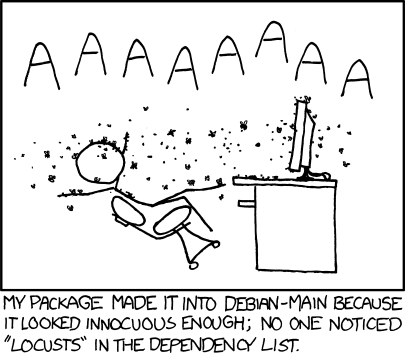
\includegraphics[width=0.6\textwidth]{images/debian_main.png}
\end{center}
\hfill xkcd 797
	

\end{frame}


%%%%%%%%%%%%%%%%%%%%%%%%%%%%%%%%%%%%%%%%%%%%%%%%%%%%%%%%%%%%%%%%%%%%%%%%%%%%%%%%
\begin{frame}[fragile]
\frametitle{Loop-carried Dependencies (1)}

Can we run these lines in parallel? \\ ~~~(initially vec[0] and vec[1] are 1)
\begin{lstlisting}[language=Rust]
let mut vec = vec![1; 32];
    /* */
vec[4] = vec[0] + 1;
vec[5] = vec[0] + 2;
\end{lstlisting}
\pause
\structure{Yes.}\\[1em]
\begin{itemize}
\item There are no dependencies between these lines.
\item However, this is not how we normally use arrays\ldots
\end{itemize}

\end{frame}
%%%%%%%%%%%%%%%%%%%%%%%%%%%%%%%%%%%%%%%%%%%%%%%%%%%%%%%%%%%%%%%%%%%%%%%%%%%%%%%%

%%%%%%%%%%%%%%%%%%%%%%%%%%%%%%%%%%%%%%%%%%%%%%%%%%%%%%%%%%%%%%%%%%%%%%%%%%%%%%%%
\begin{frame}[fragile]
\frametitle{Loop-carried Dependencies (2)}

What about this? (all elements initially 1)
\begin{lstlisting}[language=Rust]
for i in 1 .. vec.len() {
    vec[i] = vec[i-1] + 1;
}
\end{lstlisting}

\pause
\alert{No, a[2] = 3 or a[2] = 2.}\\[1em]
\begin{itemize}
\item Statements depend on previous loop iterations.
\item An example of a \structure{loop-carried dependency}.
\end{itemize}

\end{frame}
%%%%%%%%%%%%%%%%%%%%%%%%%%%%%%%%%%%%%%%%%%%%%%%%%%%%%%%%%%%%%%%%%%%%%%%%%%%%%%%%


%%%%%%%%%%%%%%%%%%%%%%%%%%%%%%%%%%%%%%%%%%%%%%%%%%%%%%%%%%%%%%%%%%%%%%%%%%%%%%%%
\begin{frame}[fragile]
\frametitle{Larger example: Loop-carried Dependencies}
{\small
\begin{lstlisting}[language=Rust]
// Repeatedly square input, return number of iterations before
// absolute value exceeds 4, or 1000, whichever is smaller.
fn mandelbrot(x0: f64, y0: f64) -> i32 {
    let mut iterations = 0;
    let mut x = x0;
    let mut y = y0;
    let mut x_squared = x * x;
    let mut y_squared = y * y;
    while (x_squared + y_squared < 4f64) && (iterations < 1000) {
        y = 2f64 * x * y + y0;
        x = x_squared - y_squared + x0;
        x_squared = x * x;
        y_squared = y * y;
        iterations += 1;
    }
    return iterations;
}
\end{lstlisting}
}
How can we parallelize this? \\
\pause
\begin{itemize}
\item Run {\tt mandelbrot} sequentially for each point, but parallelize
different point computations.
\end{itemize}
\end{frame}
%%%%%%%%%%%%%%%%%%%%%%%%%%%%%%%%%%%%%%%%%%%%%%%%%%%%%%%%%%%%%%%%%%%%%%%%%%%%%%%%


\begin{frame}[fragile]
\frametitle{Stride}

 Now consider this example---is it parallelizable? (Again, all elements initially 1.)

\begin{lstlisting}[language=C]
for i in 4 .. vec.len() {
    vec[i] = vec[i-4] + 1;
}
\end{lstlisting}

\pause

Yes, to a degree. We can execute 4 statements in parallel at a time:
\begin{itemize}
  \item \texttt{vec[4] = vec[0] + 1, vec[8] = vec[4] + 1}
  \item \texttt{vec[5] = vec[1] + 1, vec[9] = vec[5] + 1}
  \item \texttt{vec[6] = vec[2] + 1, vec[10] = vec[6] + 1}
  \item \texttt{vec[7] = vec[3] + 1, vec[11] = vec[7] + 1}
\end{itemize}  
We can say that the array accesses have stride 4

\end{frame}



%%%%%%%%%%%%%%%%%%%%%%%%%%%%%%%%%%%%%%%%%%%%%%%%%%%%%%%%%%%%%%%%%%%%%%%%%%%%%%%%
\begin{frame}[fragile]
\frametitle{Memory-carried Dependencies}

Dependencies limit the amount of parallelization.

\begin{lstlisting}[language=Rust]
let mut acct: Account = Account {
    balance: 0.0f32
};
f(&mut acct);
g(&mut acct);

/* */

fn f (a: &mut Account) {
    a.balance += 50.0f32;
}
fn g (a: &mut Account) {
    a.balance *= 1.01f32;
}
\end{lstlisting}

What are the possible outcomes after executing {\tt g()} and {\tt f()}


\end{frame}
%%%%%%%%%%%%%%%%%%%%%%%%%%%%%%%%%%%%%%%%%%%%%%%%%%%%%%%%%%%%%%%%%%%%%%%%%%%%%%%%




%%%%%%%%%%%%%%%%%%%%%%%%%%%%%%%%%%%%%%%%%%%%%%%%%%%%%%%%%%%%%%%%%%%%%%%%%%%%%%%%



\begin{frame}
\frametitle{Summary of Memory-carried Dependencies}

Well, turns out our memory-carried dependencies are the hazards:
\begin{center}
\begin{tabular}{ll|p{2.8cm}p{3.2cm}}
& & \multicolumn{2}{c}{Second Access} \\ 
&  & \bf Read & \bf Write \\ \hline
\multirow{2}{*}{First Access} & \bf Read & No Dependency Read After Read (RAR)  & Anti-dependency Write After Read (WAR) \\[0.5em]
& \bf Write & True Dependency Read After Write (RAW) & Output Dependency Write After Write (WAW) \\
\end{tabular}
\end{center}
\end{frame}
%%%%%%%%%%%%%%%%%%%%%%%%%%%%%%%%%%%%%%%%%%%%%%%%%%%%%%%%%%%%%%%%%%%%%%%%%%%%%%%%



%%%%%%%%%%%%%%%%%%%%%%%%%%%%%%%%%%%%%%%%%%%%%%%%%%%%%%%%%%%%%%%%%%%%%%%%%%%%%%%%
\begin{frame}
  \frametitle{Critical Paths}

  

  Should be familiar with critical paths from other courses (Gantt charts).\\[1em]

  Consider the following diagram (edges are tasks):

\begin{center}
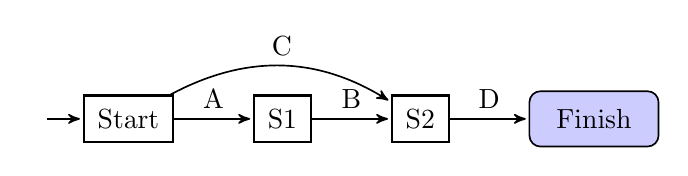
\begin{tikzpicture}[->,>=stealth',shorten >=1pt,auto,column sep=2.2cm,
                    semithick,initial text=]
  \node[initial,block] (s0) {Start};
  \node[block] (s1) [right=of s0] {S1};
  \node[block] (s2) [right=of s1] {S2};
  \node[bw] (s3) [right=of s2] {Finish};

  \path (s0) edge node {A} (s1)
        (s1) edge node {B} (s2)
        (s2) edge node {D} (s3)
        (s0) edge[bend left=30] node {C} (s2);
\end{tikzpicture}
\end{center}

  \begin{itemize}
    \item B depends on A, C has no dependencies, and D depends on B and C.
    \item Can execute A-then-B in parallel with C.
    \item Keep dependencies in mind when calculating speedups for more
      complex programs.
  \end{itemize}
  
\end{frame}
%%%%%%%%%%%%%%%%%%%%%%%%%%%%%%%%%%%%%%%%%%%%%%%%%%%%%%%%%%%%%%%%%%%%%%%%%%%%%%%%


%%%%%%%%%%%%%%%%%%%%%%%%%%%%%%%%%%%%%%%%%%%%%%%%%%%%%%%%%%%%%%%%%%%%%%%%%%%%%%%%
\begin{frame}
  \frametitle{Breaking Dependencies}

  
  \structure{Speculation}: architects use it to predict
      branch targets.
  
  \begin{center}
  	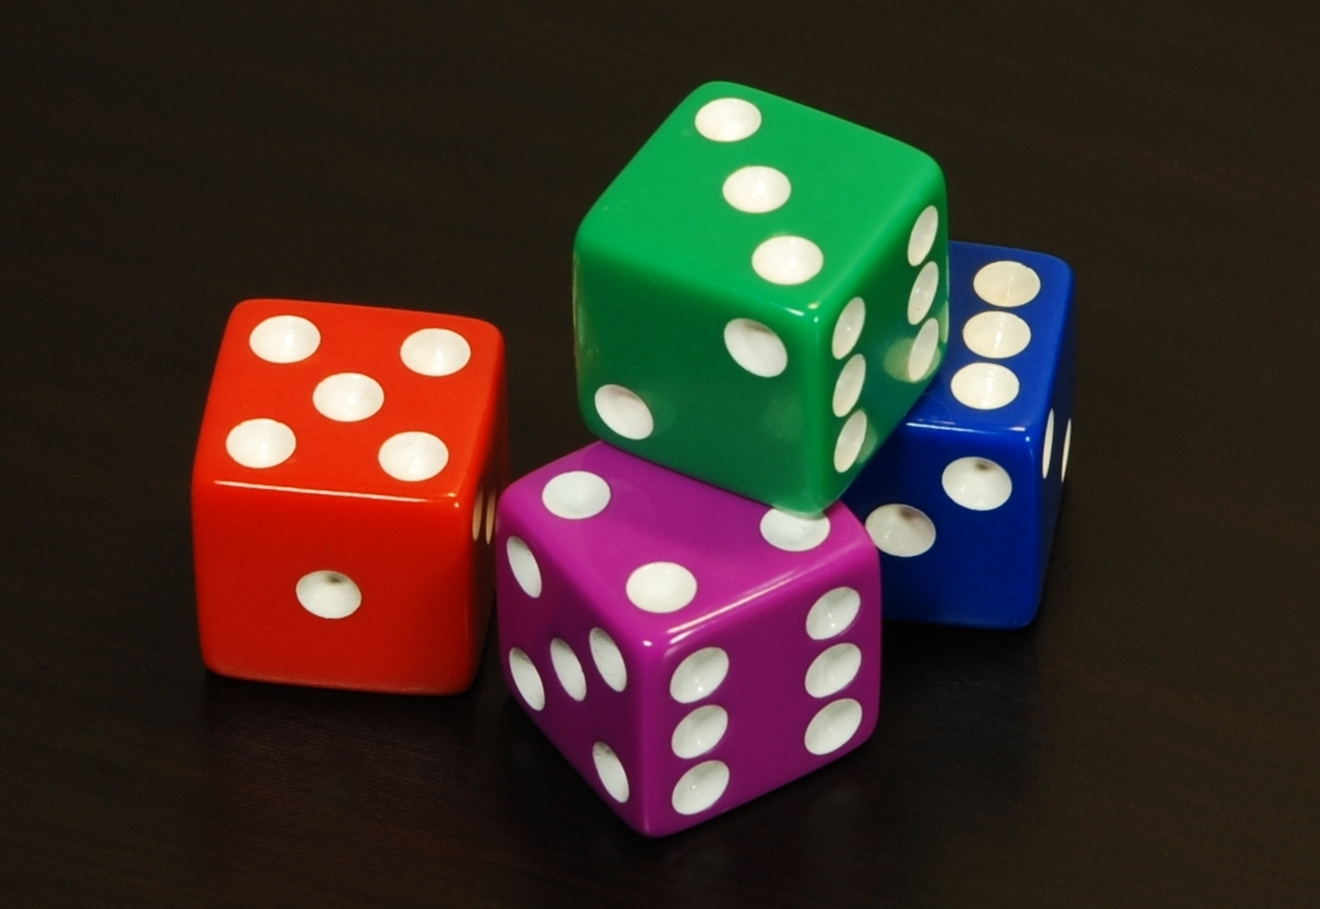
\includegraphics[width=0.5\textwidth]{images/6sided_dice.jpg}
  \end{center}
  	\hfill Image Credit: Diacritica

Roll the dice and see how we do!

\end{frame}


\begin{frame}
\frametitle{Coffee Analogy}

\begin{center}
	
\includegraphics[width=0.5\textwidth]{images/tims.jpg}
\end{center}

If you're a regular, can they guess your order?

And how much time would they save?

\end{frame}

  

\begin{frame}
\frametitle{Breaking Dependencies}

We need not wait for the branch to be evaluated.

We'll use speculation at a coarser-grained level: speculatively parallelize code.

Two ways: \alert{speculative execution} and
      \alert{value speculation}.
  
\end{frame}
%%%%%%%%%%%%%%%%%%%%%%%%%%%%%%%%%%%%%%%%%%%%%%%%%%%%%%%%%%%%%%%%%%%%%%%%%%%%%%%%




%%%%%%%%%%%%%%%%%%%%%%%%%%%%%%%%%%%%%%%%%%%%%%%%%%%%%%%%%%%%%%%%%%%%%%%%%%%%%%%%
\begin{frame}[fragile]
  \frametitle{Speculative Execution: Example}

  
Consider the following code:
  
\begin{lstlisting}[language=Rust]
fn do_work(x: i32, y: i32, threshold: i32) -> i32 {
    let val = long_calculation(x, y);
    if val > threshold {
        return val + second_long_calculation(x, y);
    }
    return val;
}
\end{lstlisting}

  Will we need to run {\tt second\_long\_calculation}?
  \vfill  
  \begin{itemize}
    \item<2> OK, so: could we execute {\tt long\_calculation} and {\tt second\_long\_calculation}
      in parallel if we didn't have the conditional?
  \end{itemize}
  
\end{frame}
%%%%%%%%%%%%%%%%%%%%%%%%%%%%%%%%%%%%%%%%%%%%%%%%%%%%%%%%%%%%%%%%%%%%%%%%%%%%%%%%

%%%%%%%%%%%%%%%%%%%%%%%%%%%%%%%%%%%%%%%%%%%%%%%%%%%%%%%%%%%%%%%%%%%%%%%%%%%%%%%%
\begin{frame}[fragile]
  \frametitle{Speculative Execution: Assume No Conditional}

  
  Yes, we could parallelize them. Consider this code:
    
\begin{lstlisting}[language=Rust]
fn do_work(x: i32, y: i32, threshold: i32) -> i32 {
    let t1 = thread::spawn(move || {
        return long_calculation(x, y);
    });
    let t2 = thread::spawn(move || {
        return second_long_calculation(x, y);
    });
    let val = t1.join().unwrap();
    let v2 = t2.join().unwrap();
    if val > threshold {
        return val + v2;
    }
    return val;
}
\end{lstlisting}

  We do both the calculations in parallel and return the same result as before.
  
    \begin{itemize}
    \item What are we assuming about {\tt long\_calculation} and
{\tt second\_long\_calculation}?
  \end{itemize}


\end{frame}

\begin{frame}[fragile]
\frametitle{Can We Improve?}

The current thread is a valid thread for doing work and we don't have to create two threads and join two threads. 

We can create one and maybe have less overhead.

\begin{lstlisting}[language=Rust]
fn do_work(x: i32, y: i32, threshold: i32) -> i32 {
    let t1 = thread::spawn(move || {
        return second_long_calculation(x, y);
    });
    let val = long_calculation(x, y);
    let v2 = t1.join().unwrap();
    if val > threshold {
        return val + v2;
    }
    return val;
}
\end{lstlisting}


\end{frame}

\begin{frame}
\frametitle{Check Assumptions}
  
  $T_1$: time to run {\tt long\_calculation}.

  $T_2$: time to run {\tt second\_long\_calculation}.

  $p$: probability that {\tt second\_long\_calculation} executes.\\[1em]

  In the normal case we have:
    \[T_{\mbox{\scriptsize normal}} = T_1 + pT_2.\]

  $S$: synchronization overhead.\\
  Our speculative code takes:
    \[ T_{\mbox{\scriptsize speculative}} = \mbox{max}(T_1, T_2) + S.\]

    \structure{Exercise.} When is speculative code faster? Slower? \\ How could you improve it?

  
\end{frame}
%%%%%%%%%%%%%%%%%%%%%%%%%%%%%%%%%%%%%%%%%%%%%%%%%%%%%%%%%%%%%%%%%%%%%%%%%%%%%%%%

%%%%%%%%%%%%%%%%%%%%%%%%%%%%%%%%%%%%%%%%%%%%%%%%%%%%%%%%%%%%%%%%%%%%%%%%%%%%%%%%
\begin{frame}[fragile]
  \frametitle{Shortcomings of Speculative Execution}

  
  Consider the following code:
  
\begin{lstlisting}[language=Rust]
fn do_other_work(x: i32, y: i32) -> i32 {
    let val = long_calculation(x, y);
    return second_long_calculation(val);
}
\end{lstlisting}

  Now we have a true dependency; can't use speculative~execution.\\[1em]

  But: if the value is predictable, we can execute
      {\tt second\_long\_calculation} using the predicted value.\\[1em]

  This is \structure{value speculation}.
  
\end{frame}
%%%%%%%%%%%%%%%%%%%%%%%%%%%%%%%%%%%%%%%%%%%%%%%%%%%%%%%%%%%%%%%%%%%%%%%%%%%%%%%%

%%%%%%%%%%%%%%%%%%%%%%%%%%%%%%%%%%%%%%%%%%%%%%%%%%%%%%%%%%%%%%%%%%%%%%%%%%%%%%%%
\begin{frame}[fragile]
  \frametitle{Value Speculation Implementation}
  
  This code does value speculation:

\begin{lstlisting}[language=Rust]
fn do_other_work(x: i32, y: i32, last_value: i32) -> i32 {
    let t = thread::spawn(move || {
        return second_long_calculation(last_value);
    });
    let val = long_calculation(x, y);
    let v2 = t.join().unwrap();
    if val == last_value {
        return v2;
    }
    return second_long_calculation(val);
}
\end{lstlisting}


  Note: this is like memoization (plus parallelization).
  
\end{frame}
%%%%%%%%%%%%%%%%%%%%%%%%%%%%%%%%%%%%%%%%%%%%%%%%%%%%%%%%%%%%%%%%%%%%%%%%%%%%%%%%

%%%%%%%%%%%%%%%%%%%%%%%%%%%%%%%%%%%%%%%%%%%%%%%%%%%%%%%%%%%%%%%%%%%%%%%%%%%%%%%%
\begin{frame}
  \frametitle{Estimating Impact of Value Speculation}

  
  $T_1$: time to run {\tt long\_calculation}.

  $T_2$: time to run {\tt second\_long\_calculation}.

  $p$: probability that {\tt second\_long\_calculation} executes again.

  $S$: synchronization overhead.\\[1em]

  In the normal case, we have:
    \[ T = T_1 +T_2.\]

  This speculative code takes:
    \[ T = \mbox{max}(T_1, T_2) + S + pT_2.\]

    \structure{Exercise.} Again, when is speculative code faster? Slower? How could you improve it?

  
\end{frame}
%%%%%%%%%%%%%%%%%%%%%%%%%%%%%%%%%%%%%%%%%%%%%%%%%%%%%%%%%%%%%%%%%%%%%%%%%%%%%%%%

%%%%%%%%%%%%%%%%%%%%%%%%%%%%%%%%%%%%%%%%%%%%%%%%%%%%%%%%%%%%%%%%%%%%%%%%%%%%%%%%
\begin{frame}
  \frametitle{When Can We Speculate?}

  
  Required conditions for safety:

  \begin{itemize}
    \item {\tt long\_calculation} and {\tt second\_long\_calculation} must not call
      each other.
    \item {\tt second\_long\_calculation} must not depend on
      any values set or modified by {\tt long\_calculation}.
    \item The return value of {\tt long\_calculation} must be deterministic.
  \end{itemize}

  General warning: Consider \structure{side effects} of function calls.
  
\end{frame}
%%%%%%%%%%%%%%%%%%%%%%%%%%%%%%%%%%%%%%%%%%%%%%%%%%%%%%%%%%%%%%%%%%%%%%%%%%%%%%%%



\begin{frame}
\frametitle{Side Effects}

\begin{center}
	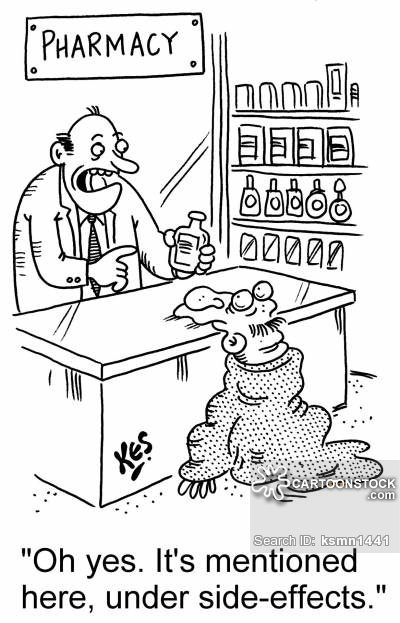
\includegraphics[width=0.4\textwidth]{images/side-effects.jpg}
\end{center}
\hfill Image Credit: Kes, Cartoonstock


\end{frame}


\begin{frame}
\frametitle{Side Effects}

As a general warning: Consider the \alert{side effects} of function calls. 

They have a big impact on parallelism. Side effects are problematic, but why? 

For one thing they're kind of unpredictable. 

Side effects are changes in state that do not depend on the function input. 

\end{frame}


\begin{frame}
\frametitle{Side Effects}

Calling a function or expression has a side effect if it has some visible effect on the outside world. 

Some things necessarily have side effects, like printing to the console. 

Others are side effects which may be avoidable if we can help it, like modifying a global variable.

\end{frame}




\begin{frame}
\frametitle{Software Transactional Memory}

\begin{center}
	
\includegraphics[width=0.5\textwidth]{images/timetravel.jpg}
\end{center}


\end{frame}


%%%%%%%%%%%%%%%%%%%%%%%%%%%%%%%%%%%%%%%%%%%%%%%%%%%%%%%%%%%%%%%%%%%%%%%%%%%%%%%%
\begin{frame}
  \frametitle{STM: Introduction}


    Instead of programming with locks, we have transactions on memory.
      \begin{itemize}
        \item Analogous to database transactions
      \end{itemize}
    An old idea; recently saw some renewed interest.\\[1em]

    A series of memory operations either all succeed; or \\ \qquad
     all fail (and get
      rolled back), and are later retried.

\end{frame}
%%%%%%%%%%%%%%%%%%%%%%%%%%%%%%%%%%%%%%%%%%%%%%%%%%%%%%%%%%%%%%%%%%%%%%%%%%%%%%%%

%%%%%%%%%%%%%%%%%%%%%%%%%%%%%%%%%%%%%%%%%%%%%%%%%%%%%%%%%%%%%%%%%%%%%%%%%%%%%%%%
\begin{frame}
  \frametitle{STM: Benefits}


    Simple programming model: need not worry about lock
      granularity or deadlocks.\\[1em]

    Just group lines of code that should logically be one operation
      in an {\tt atomic} block!\\[1em]

    It is the responsibility of the implementer to ensure the code
      operates as an atomic transaction.

\end{frame}
%%%%%%%%%%%%%%%%%%%%%%%%%%%%%%%%%%%%%%%%%%%%%%%%%%%%%%%%%%%%%%%%%%%%%%%%%%%%%%%%


\begin{frame}[fragile]
\frametitle{STM Example}

Set up a transaction with an atomic block:

\begin{lstlisting}[language=Rust]
let x = atomically(|trans| {
    var.write(trans, 42)?; // Pass failure to parent.
    var.read(trans) // Return the value saved in var.
});
\end{lstlisting}


\end{frame}


%%%%%%%%%%%%%%%%%%%%%%%%%%%%%%%%%%%%%%%%%%%%%%%%%%%%%%%%%%%%%%%%%%%%%%%%%%%%%%%%
\begin{frame}[fragile]
  \frametitle{STM: Implementing a Motivating Example}


\begin{lstlisting}[language=Rust]
struct Account {
    balance: TVar<f32>,
}

fn transfer_funds(sender: &mut Account, receiver: &mut Account, amount: f32) {
    atomically(|tx| {
        let sender_balance = sender.balance.read(tx)?;
        let receiver_balance = receiver.balance.read(tx)?;
        sender.balance.write(tx, sender_balance - amount)?;
        receiver.balance.write(tx, receiver_balance + amount)?;
        Ok(0)
    });
}
\end{lstlisting}

[Note: bank transfers aren't actually atomic!]\\[1em]

With STM, we do not have to worry about remembering to acquire locks,
      or about deadlocks.

\end{frame}
%%%%%%%%%%%%%%%%%%%%%%%%%%%%%%%%%%%%%%%%%%%%%%%%%%%%%%%%%%%%%%%%%%%%%%%%%%%%%%%% 

%%%%%%%%%%%%%%%%%%%%%%%%%%%%%%%%%%%%%%%%%%%%%%%%%%%%%%%%%%%%%%%%%%%%%%%%%%%%%%%%
\begin{frame}
  \frametitle{STM: Drawbacks}


    Rollback is key to STM. \\
     \qquad But, some things cannot be rolled back. \\
     \qquad (write to the screen, send packet over network)\\[1em]

    Nested transactions. \\
     \qquad What if an inner transaction succeeds, \\ yet the
      transaction aborts? \\[1em]

    Limited transaction size: \\
 \qquad Most implementations (especially
    all-hardware) \\ have a limited transaction size.

\end{frame}
%%%%%%%%%%%%%%%%%%%%%%%%%%%%%%%%%%%%%%%%%%%%%%%%%%%%%%%%%%%%%%%%%%%%%%%%%%%%%%%%

%%%%%%%%%%%%%%%%%%%%%%%%%%%%%%%%%%%%%%%%%%%%%%%%%%%%%%%%%%%%%%%%%%%%%%%%%%%%%%%%
\begin{frame}
  \frametitle{Basic STM Implementation (Software)}


    In all atomic blocks, record all reads/writes to a log.\\[1em]
    At the end of the block, running thread verifies that no other threads
      have modified any values read.\\[1em]
    If validation is successful, changes are {\bf committed}.\\
    Otherwise, the block is {\bf aborted} and re-executed.\\[2em]

  Note: Hardware implementations exist too.



\end{frame}
%%%%%%%%%%%%%%%%%%%%%%%%%%%%%%%%%%%%%%%%%%%%%%%%%%%%%%%%%%%%%%%%%%%%%%%%%%%%%%%%

%%%%%%%%%%%%%%%%%%%%%%%%%%%%%%%%%%%%%%%%%%%%%%%%%%%%%%%%%%%%%%%%%%%%%%%%%%%%%%%%
\begin{frame}[fragile]
  \frametitle{Basic STM Implementation Issues}


    Since you don't protect against dataraces (just rollback),\\
      a datarace may trigger a fatal error in your program.

\begin{tabular}{r|l}
\begin{minipage}{.46\textwidth}
\begin{lstlisting}[language=Rust]
fn what_could_go_wrong(x: TVar<i32>, y: TVar<i32>) {
    atomically(|t| {
        let old_x = x.read(t)?;
        let old_y = y.read(t)?;
        x.write(t, old_x + 1);
        y.write(t, old_y + 1);
        Ok(0)
    });
}
\end{lstlisting}
\end{minipage}
&
\begin{minipage}{.52\textwidth}
\begin{lstlisting}[language=Rust]
fn oh_no(x: TVar<i32>, y: TVar<i32>) {
    atomically(|transaction| {
        if x.read(transaction)? != y.read(transaction)? {
            loop { /* Cursed Thread */}
        }
        Ok(0)
    });
}
\end{lstlisting}
\end{minipage}
\end{tabular}

 In this silly example, assume initially {\tt x = y}. You may think the
      code will not go into an infinite loop, but it can.

\end{frame}
%%%%%%%%%%%%%%%%%%%%%%%%%%%%%%%%%%%%%%%%%%%%%%%%%%%%%%%%%%%%%%%%%%%%%%%%%%%%%%%%


%%%%%%%%%%%%%%%%%%%%%%%%%%%%%%%%%%%%%%%%%%%%%%%%%%%%%%%%%%%%%%%%%%%%%%%%%%%%%%%%
\begin{frame}
  \frametitle{STM Summary}


     Software Transactional Memory gives another approach to
      parallelism: \\ \qquad no need to deal with locks and their associated problems.

     Currently slow, but a lot of research is going into improving it. (futile?)

     Operates by either completing an atomic block, or retrying (by rolling
      back) until it successfully completes.

\end{frame}


\end{document}

